\begin{frame}{Коммуникационные задачи}

    \begin{center}
    	\onslide<1->{
    \tikzstyle{op1} = [opacity = 0]
    \tikzstyle{op2} = [opacity = 0]
    \tikzstyle{op3} = [opacity = 0]
    \tikzstyle{op4} = [opacity = 0]
}
\only<2->{\tikzstyle{op2} = [opacity = 1]}
\only<3->{\tikzstyle{op3} = [opacity = 1]}
\only<4->{\tikzstyle{op4} = [opacity = 1]}

\begin{tikzpicture}[black]
    \node[police, female, minimum size = 1.5cm] (alice) at (0, 0) {};
    \node[jester, mirrored, minimum size = 1.5cm] (bob) at (7, 0) {};
    \node[above = 0.3 of alice] {$x \in U$};
    \node[above = 0.3 of bob] {$y \in V$};

    \path (alice.east) -- (bob.west) node[midway, above = 2.3] {\Large $f(x, y) = ?$};
    \draw[op2, ->, thick] ($(alice.east) + (0.3, 1)$) -- ($(bob.west) + (-0.3, 1)$) node[midway, above] {$r_1 = a(x)$};
    \draw[op3, <-, thick] ($(alice.east) + (0.3, 0.2)$) -- ($(bob.west) + (-0.3, 0.2)$) node[midway, above] {$r_2 = b(y,
        r_1)$};
    \draw[op4, ->, thick] ($(alice.east) + (0.3, -0.2)$) -- ($(bob.west) + (-0.3, -0.2)$);
    \draw[op4, ->, thick] ($(alice.east) + (0.3, -0.6)$) -- ($(bob.west) + (-0.3, -0.6)$) node[midway, below] {$\vdots$};
\end{tikzpicture}    
    \end{center}

    \pause
    \pause
    \pause
	\pause

    \deftext{Коммуникационная сложность} функции $f$~--- минимально возможная длина всех сообщений в
    протоколе.
\end{frame}


\begin{frame}{Примеры коммуникационных задач}
    
    $x$ и $y$~--- строки длины $n$ из нулей и единиц
            
    \begin{overlayarea}{\textwidth}{10cm}
        \begin{enumerate}
            \item $\Avg(x, y) \coloneqq \sum\limits_{i = 1}^{n} i \cdot (x_i + y_i)$, где
                $x_i, y_i$~--- соответствующие биты $x$ и $y$;
        \suspend{enumerate}

        \pause
        \only<2>{
            $$
                \Avg(x, y) \coloneqq \sum\limits_{i = 1}^{n} i \cdot x_i +
                \sum\limits_{i = 1}^{n} i \cdot y_i
            $$
        }

        \pause
        \resume{enumerate}
            \item $\EQ(x, y) \coloneqq x \stackrel{?}{=} y$;
        \suspend{enumerate}

        \only<4->{
            \begin{center}
                \tikzstyle{inner} = [circle, minimum size = 0.3cm, draw, inner sep = 0.1pt]
\tikzstyle{gstyle} = [fill = green]
\tikzstyle{rstyle} = [fill = red]
\tikzstyle{ed} = [->, draw]
\tikzstyle{ops} = [alt=<{#1-}>{opacity = 1}{opacity = 0}]
\tikzstyle{opstyle} = [inner, ops = #1]
\tikzstyle{oped} = [ed, ops = #1]
\tikzstyle{gstyle} = [alt=<{#1}>{fill = green}{}]
\tikzstyle{rstyle} = [alt=<{#1}>{red!90!black}{}]
\tikzstyle{snakestyle} = [
    alt=<{#1}>{
        decorate,
        decoration = {
            snake,
            amplitude = 0.4mm,
            segment length = 2mm,
            post length = 1mm
        }
    }{}]


    
\begin{tikzpicture}[>=latex]
    
    \node[inner, gstyle = 10] (a) at (0, 0) {\scriptsize $a$};
    \node[opstyle = 6, gstyle = 11] (b) at (-2, -0.8) {\scriptsize $b$};
    \node[opstyle = 6] (c) at (2, -0.8) {\scriptsize $a$};
    \node[opstyle = 8] (d) at (-2.9, -1.6) {};
    \node[ops = 8, below = 4pt] at (d) {\scriptsize <<да>>};
    \node[opstyle = 8, gstyle = 12] (e) at (-1.1, -1.6) {\scriptsize $b$};
    \node[opstyle = 9] (f) at (1.1, -1.6) {};
    \node[ops = 9, below = 4pt] at (f) at (1.1, -1.6) {\scriptsize <<нет>>};
    \node[opstyle = 9] (g) at (2.9, -1.6) {\scriptsize $b$};

    \node[opstyle = 9] (h) at (-1.6, -2.4) {};
    \node[ops = 9, below = 4pt] at (h) {\scriptsize <<нет>>};
	\node[opstyle = 9, gstyle = 13] (i) at (-0.6, -2.4) {\scriptsize $a$};
    
    \node[opstyle = 9] (j) at (2.4, -2.4) {};
    \node[ops = 9, below = 4pt] at (j) {\scriptsize <<нет>>};
    \node[opstyle = 9] (k) at (3.4, -2.4) {};
    \node[ops = 9, below = 4pt] at (k) {\scriptsize <<да>>};

    \node[opstyle = 9, gstyle = 14] (l) at (-1, -3.2) {};
    \node[ops = 9, below = 4pt] at (l) {\scriptsize <<да>>};
    \node[opstyle = 9] (m) at (-0.2, -3.2) {};
    \node[ops = 9, below = 4pt] at (m) {\scriptsize <<нет>>};
    
    \draw[oped = 5, rstyle = {16-17}, snakestyle = 17] (a) -- (b);
    \draw[oped = 5] (a) -- (c);
    \draw[oped = 7] (b) -- (d);
    \draw[oped = 7, rstyle = {16-17}] (b) -- (e);
    \draw[oped = 9] (c) -- (f);
    \draw[oped = 9] (c) -- (g);
    \draw[oped = 9] (e) -- (h);
    \draw[oped = 9, rstyle = {16-17}] (e) -- (i);
    \draw[oped = 9] (g) -- (j);
    \draw[oped = 9] (g) -- (k);
    \draw[oped = 9, rstyle = {16-17}, snakestyle = 17] (i) -- (l);
    \draw[oped = 9] (i) -- (m);
\end{tikzpicture}
            \end{center}

            \pause
            \pause
            \pause
            \pause
            \pause
            \pause
            \pause
            \pause
            \pause
            \pause
            \pause
            \pause

            \only<16-18>{
                \begin{center}
                    $(\alpha, \alpha)$ \qquad $(\beta, \beta)$
                \end{center}
            }
            \only<18>{
                \begin{center}
                    $(\alpha, \beta)$ \qquad $(\beta, \alpha)$
                \end{center}
                }
            \only<19>{
                Для каждой пары $(\alpha, \alpha)$ должен быть свой лист $\Rightarrow$ не меньше $2^n +
                1$ листов $\Rightarrow$ глубина не меньше $n + 1$.
            }
        }

        \pause
        \pause
        \pause
        \pause
        \pause
        \resume{enumerate}
            \item $\GT(x, y) \coloneqq x \stackrel{?}{\ge} y$;
            \item $\Disj(x, y) \coloneqq x \cap y \stackrel{?}{=} \emptyset$;
        \end{enumerate}
    \end{overlayarea}
\end{frame}

\begin{frame}{Решение систем уравнений}

    Переменные $x_{i, j}$, где $i \in \{1, 2, \dots, n + 1\}$, $j \in \{1, 2, \dots, n\}$

    $x_{i, j} \in \{0, 1\}$
    \vspace{0.1cm}
    
    $
    \begin{cases}
        \prod\limits_{j = 1}^{n}(1 - x_{i, j}) = 0 & \text{для всех } i \in \{1, \dots, n + 1\} \\ 
        x_{i, j} \cdot x_{i', j} = 0 & \text{для всех } i \neq i', j \in \{1, \dots, n\}
    \end{cases}
    $

    \pause

    \vspace{0.2cm}
    \begin{minipage}{0.3\linewidth}
        \centering
        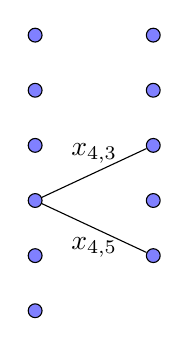
\begin{tikzpicture}[>=latex]

    \foreach \i in {1, 2, ..., 6}{
        \node[draw, circle, fill = blue!50, inner sep = 0pt, minimum size = 5pt]
            (a\i) at (0, -0.7 * \i) {};
    }

    \foreach \i in {1, 2, ..., 5}{
        \node[draw, circle, fill = blue!50, inner sep = 0pt, minimum size = 5pt]
            (b\i) at (1.5, -0.7 * \i) {};
    }
    
    \draw (a4) -- (b3) node[midway, above] {$x_{4, 3}$};
    \draw (a4) -- (b5) node[midway, below] {$x_{4, 5}$};
\end{tikzpicture}
    \end{minipage}
    \pause
    \begin{minipage}{0.68\linewidth}
        \centering
        \tikzstyle{inner} = [circle, minimum size = 0.5cm, inner sep = 0.2pt]
\tikzstyle{ed} = [->, draw]
\tikzstyle{ops} = [alt=<{#1-}>{opacity = 1}{opacity = 0}]
\tikzstyle{dotstyle} = [inner, ops = #1]
\tikzstyle{opstyle} = [inner, draw, ops = #1]
\tikzstyle{oped} = [ed, ops = #1]
\tikzstyle{gstyle} = [alt=<{#1}>{fill = green}{}]
\tikzstyle{rstyle} = [alt=<{#1}>{red!90!black}{}]
\tikzstyle{snakestyle} = [
    alt=<{#1}>{
        decorate,
        decoration = {
            snake,
            amplitude = 0.4mm,
            segment length = 2mm,
            post length = 1mm
        }
    }{}]


    
\begin{tikzpicture}[>=latex]
    \node[inner, draw] (a) at (0, 0) {$x$};
    \node[opstyle = 5] (b) at (-2, -1) {$y$};
    \node[opstyle = 5] (c) at (2, -1) {$z$};
    \node[opstyle = 7] (d) at (-2.9, -2) {};
    \node[ops = 7] (err) at (-3.5, -3) {\scriptsize <<нарушено условие>>};
    \node[opstyle = 8] (e) at (-1.1, -2) {$w$};
    \node[dotstyle = 9] (f) at (1.1, -2) {$\vdots$};
    \node[dotstyle = 9] (g) at (2.9, -2) {$\vdots$};

    \node[dotstyle = 9] (h) at (-1.9, -3) {$\vdots$};
	\node[dotstyle = 9] (i) at (-0.3, -3) {$\vdots$};
    
    
    \draw[oped = 4] (a) -- (b) node[midway, above] {$0$};
    \draw[oped = 4] (a) -- (c) node[midway, above] {$1$};
    \draw[oped = 6] (b) -- (d) node[midway, above] {$0$};
    \draw[oped = 6] (b) -- (e) node[midway, above] {$1$};
    \draw[oped = 8] (c) -- (f) node[midway, above] {$0$};
    \draw[oped = 8] (c) -- (g) node[midway, above] {$1$};
    \draw[oped = 8] (e) -- (h) node[midway, above] {$0$};
    \draw[oped = 8] (e) -- (i) node[midway, above] {$1$};
    \draw[oped = 7, very thick, red] (err) -- (d);
\end{tikzpicture}
    \end{minipage}
    
\end{frame}

\begin{frame}{Задача поиска противоречия $\Search$}

    Разделим переменные между Алисой и Бобом. $C_i(x, y)$~--- набор уравнений.
    
    Цель: по значениям $\alpha$ и $\beta$ найти $i$, что $C_i(\alpha, \beta)$

    \pause
    \vspace{0.2cm}
    \begin{minipage}{0.5\linewidth}
        \centering
        \tikzstyle{inner} = [circle, minimum size = 0.2cm, inner sep = 0.1pt]
\tikzstyle{gstyle} = [fill = green]
\tikzstyle{rstyle} = [fill = red]
\tikzstyle{ed} = [->, draw]
\tikzstyle{ops} = [alt=<{#1-}>{opacity = 1}{opacity = 0}]
\tikzstyle{dotstyle} = [inner, ops = #1]
\tikzstyle{opstyle} = [inner, draw, ops = #1]
\tikzstyle{oped} = [ed, ops = #1]
\tikzstyle{gstyle} = [alt=<{#1}>{fill = green}{}]
\tikzstyle{rstyle} = [alt=<{#1}>{red!90!black}{}]
\tikzstyle{snakestyle} = [
    alt=<{#1}>{
        decorate,
        decoration = {
            snake,
            amplitude = 0.4mm,
            segment length = 2mm,
            post length = 1mm
        }
    }{}]


    
\begin{tikzpicture}[>=latex]
    \node[inner, draw, gstyle = 4] (a) at (0, 0) {};
    \node[inner, draw, gstyle = 5] (b) at (-1.5, -0.8) {};
    \node[inner, draw] (c) at (1.5, -0.8) {};
    \node[inner] (d) at (-2, -1.6) {\scriptsize $\vdots$};
    \node[inner, draw, gstyle = 6] (e) at (-1, -1.6) {};
    \node[inner] (f) at (1, -1.6) {\scriptsize $\vdots$};
    \node[inner, draw] (g) at (2, -1.6) {};

    \node[inner] (h) at (-1.4, -2.4) {\scriptsize $\vdots$};
	\node[inner, draw] (i) at (-0.6, -2.4) {};
    
    \node[inner] (j) at (1.6, -2.4) {\scriptsize $\vdots$};
    \node[inner] (k) at (2.4, -2.4) {\scriptsize $\vdots$};

    \node[inner] (l) at (-1, -3.2) {\scriptsize $\vdots$};
    \node[inner] (m) at (-0.2, -3.2) {\scriptsize $\vdots$};
    
    \draw[ed, rstyle = {9}] (a) -- (b);
    \draw[ed] (a) -- (c);
    \draw[ed] (b) -- (d);
    \draw[ed, rstyle = {9}] (b) -- (e);
    \draw[ed] (c) -- (f);
    \draw[ed] (c) -- (g);
    \draw[ed] (e) -- (h);
    \draw[ed] (e) -- (i);
    \draw[ed] (g) -- (j);
    \draw[ed] (g) -- (k);
    \draw[ed] (i) -- (l);
    \draw[ed] (i) -- (m);

    \path (e) ++(90:0.4) coordinate (p1);
    \path (m) ++(-30:0.4) coordinate (p2);
    \path (-1.8, -3.2) ++(-150:0.4) coordinate (p3);
    
    \draw[
        orange,
        thick,
        fill = orange!50,
        rounded corners = 5pt,
        alt = <{7-}>{opacity = 0.3}{opacity = 0}] (p1) -- (p2) -- (p3) -- cycle;
\end{tikzpicture}
    \end{minipage}
    \pause
    \begin{minipage}{0.48\linewidth}
        \begin{enumerate}
            \item Найдем такую вершину $v$, что $\frac{1}{3} |T| \le |T_v| \le \frac{2}{3} |T|$.
                \pause
                \pause
                \pause
                \pause
                \pause
            \item Алиса и Боб могут за $2$ бита проверить придут ли они в нее.
                \pause
                \pause
            \item Перейдем либо в $T_v$, либо в $T \setminus T_v$.
        \end{enumerate}
        \pause
        Итог: достаточно $2 \log_{3 / 2} t$ битов коммуникации.
    \end{minipage}
    
    \pause

    \begin{theorem}
        Если $\Search$ для системы $C$ требует $k$ битов коммуникации, то алгоритм <<расщепления>> будет
        работать время $2^{\varepsilon k}$ для некоторого $k$.
    \end{theorem}
\end{frame}